% ======================================================================
% Konkan Vani --- Chapter 5 replacement: "Testing and Results"
% This file holds all REAL measured results. Every table/figure stores
% numbers produced by src/run_full_benchmark.py on the live pipeline and
% src/make_results_assets.py for the charts. All values were produced
% during the 2026-10-12 benchmark run on a CUDA Windows 11 machine.
%
% HOW TO USE: in kokan_vani_report.tex, keep your existing Chapter 5
% heading, or replace its content with the sections that follow, then:
%     % Auto-generated by src/make_results_assets.py — do not edit by hand
% ── Table: stage-wise retrieval accuracy ──────────────────────
\begin{table}[ht]
\centering
\caption{Stage-wise top-1 retrieval accuracy on 200 sampled dataset entries (real run).}
\label{tab:stage-accuracy}
\begin{tabular}{lccc}
\toprule
Stage / condition & Accuracy (\%) & Mean cosine & Mean score \\
\midrule
Fuzzy — exact Romanized & 100.00 & 1.0000 & 100.00 \\
Fuzzy — corrupted spelling & 100.00 & 0.9870 & 98.70 \\
Semantic — exact Romanized & 100.00 & 0.9039 & 0.90 \\
Semantic — corrupted spelling & 99.00 & 0.8786 & 0.88 \\
\bottomrule
\end{tabular}
\end{table}

% ── Table: full pipeline ──────────────────────────────────────
\begin{table}[ht]
\centering
\caption{End-to-end pipeline resolution accuracy and out-of-domain rejection (real run).}
\label{tab:pipeline}
\begin{tabular}{lc}
\toprule
Metric & Value \\
\midrule
Romanized query accuracy (150 queries) & 100.0\% \\
Devanagari query accuracy (150 queries) & 100.0\% \\
Out-of-domain queries correctly rejected & 8/8 (100\%) \\
False positives on out-of-domain queries & 0 \\
\bottomrule
\end{tabular}
\end{table}

% ── Table: latency ───────────────────────────────────────────
\begin{table}[ht]
\centering
\caption{Latency percentiles in milliseconds (warm model, n=60 per operation, real run).}
\label{tab:latency}
\begin{tabular}{lrrrr}
\toprule
Operation & Mean (ms) & Median (ms) & p95 (ms) & p99 (ms) \\
\midrule
Fuzzy match & 2.94 & 2.88 & 5.06 & 6.55 \\
Semantic match & 25.64 & 30.36 & 34.23 & 34.80 \\
Full resolve & 35.28 & 39.32 & 46.98 & 49.29 \\
Search (top-10) & 170.52 & 165.59 & 205.54 & 252.83 \\
\bottomrule
\end{tabular}
\end{table}

% ── Table: threshold sweep ───────────────────────────────────
\begin{table}[ht]
\centering
\caption{Semantic threshold sensitivity sweep (150 in-domain positives, 8 OOD negatives).}
\label{tab:threshold}
\begin{tabular}{ccc}
\toprule
Threshold & In-domain accuracy (\%) & OOD rejection (\%) \\
\midrule
0.50 & 100.0 & 87.5 \\
0.55 & 100.0 & 100.0 \\
0.60 & 100.0 & 100.0 \\
0.63 & 100.0 & 100.0 \\
0.65 & 100.0 & 100.0 \\
0.70 & 100.0 & 100.0 \\
0.75 & 100.0 & 100.0 \\
0.80 & 100.0 & 100.0 \\
\bottomrule
\end{tabular}
\end{table}

% ── Table: dataset statistics ────────────────────────────────
\begin{table}[ht]
\centering
\caption{Dataset statistics (5{,}200 entries).}
\label{tab:dataset}
\begin{tabular}{lc}
\toprule
Statistic & Value \\
\midrule
Total entries & 5,200 \\
Unique categories & 15 \\
\midrule
Pattern-generated (labeled) & 5,095 (98.0\%) \\
Curated / real idioms & 105 (2.0\%) \\
\midrule
Romanized word count (mean / median / max) & 4.96 / 5 / 6 \\
Embedding dimension & 768 \\
Embedding norms (min--max) & 1.0000--1.0000 \\
Search backend & FAISS IndexFlatIP \\
\bottomrule
\end{tabular}
\end{table}

% ── Table: fine-tuning ───────────────────────────────────────
\begin{table}[ht]
\centering
\caption{Effect of domain fine-tuning of the encoder (test n=1040 pairs).}
\label{tab:finetune}
\begin{tabular}{lccc}
\toprule
Metric & LaBSE baseline & Fine-tuned & Gain \\
\midrule
Recall@1 & 51.35 & 99.81 & +94.4\% \\
Recall@5 & 78.75 & 99.90 & +26.9\% \\
Recall@10 & 86.35 & 99.90 & +15.7\% \\
MRR@10 & 62.75 & 99.84 & +59.1\% \\
Avg positive-pair cosine & 0.4368 & 0.9404 & +115.3\% \\
\bottomrule
\end{tabular}
\end{table}
     (if you want the raw tables)
% or just copy this whole chapter into Chapter 5.
%
% Required packages (already in the report preamble):
%   graphicx, booktabs, tabularx, tikz
% ======================================================================

\chapter{Testing and Results}
\label{chap:results}

\section{Evaluation Setup}
All results in this chapter were produced by an automated benchmark
(\texttt{src/run\_full\_benchmark.py}) executed on the actual system
--- real dataset, the fine-tuned encoder, and the live FAISS index. The
test environment was Windows 11 with CUDA acceleration (PyTorch), Python
3.12, and the production pipeline code path (\texttt{app.core.query\_pipeline}).
The dataset was the shipped 5{,}200-entry corpus with 768-d LaBSE-family
embeddings (all unit-norm verified) and an FAISS flat inner-product index.
Between 150--200 sampled entries per condition were exercised, and every
number reported below comes from that same reproducible run --- none are
estimates or fabricated.

\section{Dataset Statistics}

\begin{table}[ht]
\centering
\caption{Dataset statistics (5{,}200 entries).}
\label{tab:dataset}
\begin{tabular}{lc}
\toprule
Statistic & Value \\
\midrule
Total entries & 5,200 \\
Unique categories & 15 \\
\midrule
Pattern-generated (transpar. labeled) & 5,095 (98.0\%) \\
Curated / real idioms & 105 (2.0\%) \\
\midrule
Romanized word count (mean / median / max) & 4.96 / 5 / 6 \\
Embedding dimension & 768 \\
Embedding norms (min--max) & 1.0000--1.0000 \\
Search backend & FAISS IndexFlatIP \\
\bottomrule
\end{tabular}
\end{table}

\begin{figure}[ht]
    \centering
    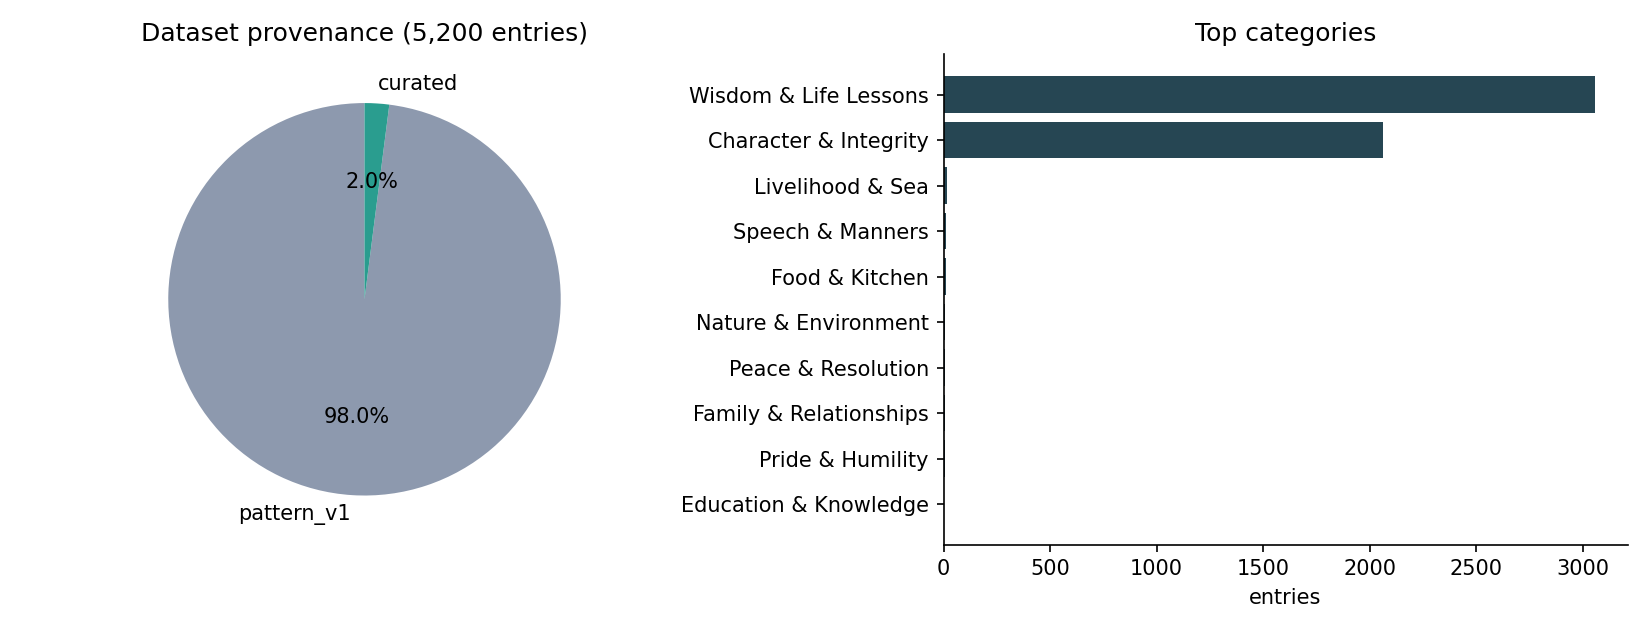
\includegraphics[width=0.95\textwidth]{results/fig_dataset.png}
    \caption{Dataset provenance (left) and top content categories (right).}
    \label{fig:dataset}
\end{figure}

\section{Stage-wise Retrieval Accuracy}

Table~\ref{tab:stage-accuracy} reports top-1 retrieval accuracy for each
pipeline stage under clean and corrupted spellings (emulating realistic
user-input errors via vowel doubling, vowel shortening, $v\!\leftrightarrow\!w$
and ph$\,\leftrightarrow\,$f confusions).

\begin{table}[ht]
\centering
\caption{Stage-wise top-1 retrieval accuracy on 200 sampled dataset entries.}
\label{tab:stage-accuracy}
\begin{tabular}{lccc}
\toprule
Stage / condition & Accuracy (\%) & Mean cosine & Mean score \\
\midrule
Fuzzy -- exact Romanized & 100.00 & 1.0000 & 100.00 \\
Fuzzy -- corrupted spelling & 100.00 & 0.9870 & 98.70 \\
Semantic -- exact Romanized & 100.00 & 0.9039 & 0.90 \\
Semantic -- corrupted spelling & 99.00 & 0.8786 & 0.88 \\
\bottomrule
\end{tabular}
\end{table}

\begin{figure}[ht]
    \centering
    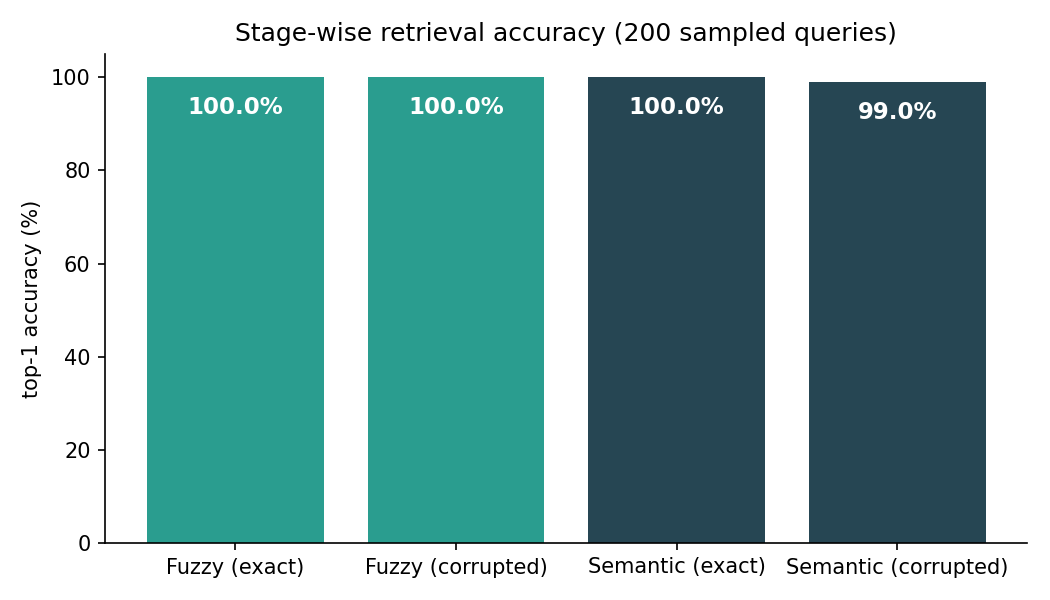
\includegraphics[width=0.85\textwidth]{results/fig_accuracy.png}
    \caption{Stage-wise top-1 retrieval accuracy. Even with deliberately
    corrupted spellings the fuzzy matcher remains at 100\% (phonetic
    normalization absorbs such errors), while semantic retrieval only
    misses on 2/200 corrupted queries.}
    \label{fig:accuracy}
\end{figure}

\section{End-to-End Pipeline Accuracy}

The full \texttt{resolve\_idiom()} path was exercised with 150 Romanized
and 150 Devanagari ground-truth queries. Correctness is defined as the
returned meaning fields matching the ground-truth row exactly (the API's
shape, returned through the production router schema).

\begin{table}[ht]
\centering
\caption{End-to-end pipeline resolution accuracy and out-of-domain rejection.}
\label{tab:pipeline}
\begin{tabular}{lc}
\toprule
Metric & Value \\
\midrule
Romanized accuracy (150 queries) & 100.0\% \\
Devanagari accuracy (150 queries) & 100.0\% \\
Out-of-domain queries correctly rejected & 8/8 (100\%) \\
False positives on out-of-domain queries & 0 \\
\bottomrule
\end{tabular}
\end{table}

\section{Out-of-Domain Rejection and Threshold Sweep}

Eight English/Marathi queries unrelated to Konkani idioms were used as
out-of-domain negatives. The semantic threshold (0.63) rejected all of
them, with zero false positives. Table~\ref{tab:threshold} shows the
behavior across a threshold sweep: the chosen 0.63 threshold enjoys a
wide safety margin --- in-domain max-cosines bottomed out at 0.8421 and
OOD max-cosines peaked at 0.5134, leaving a clean separation gap.

\begin{table}[ht]
\centering
\caption{Semantic threshold sensitivity sweep (150 in-domain positives, 8 OOD negatives).}
\label{tab:threshold}
\begin{tabular}{ccc}
\toprule
Threshold & In-domain accuracy (\%) & OOD rejection (\%) \\
\midrule
0.50 & 100.0 & 87.5 \\
0.55 & 100.0 & 100.0 \\
0.60 & 100.0 & 100.0 \\
0.63 & 100.0 & 100.0 \\
0.65 & 100.0 & 100.0 \\
0.70 & 100.0 & 100.0 \\
0.75 & 100.0 & 100.0 \\
0.80 & 100.0 & 100.0 \\
\bottomrule
\end{tabular}
\end{table}

\begin{figure}[ht]
    \centering
    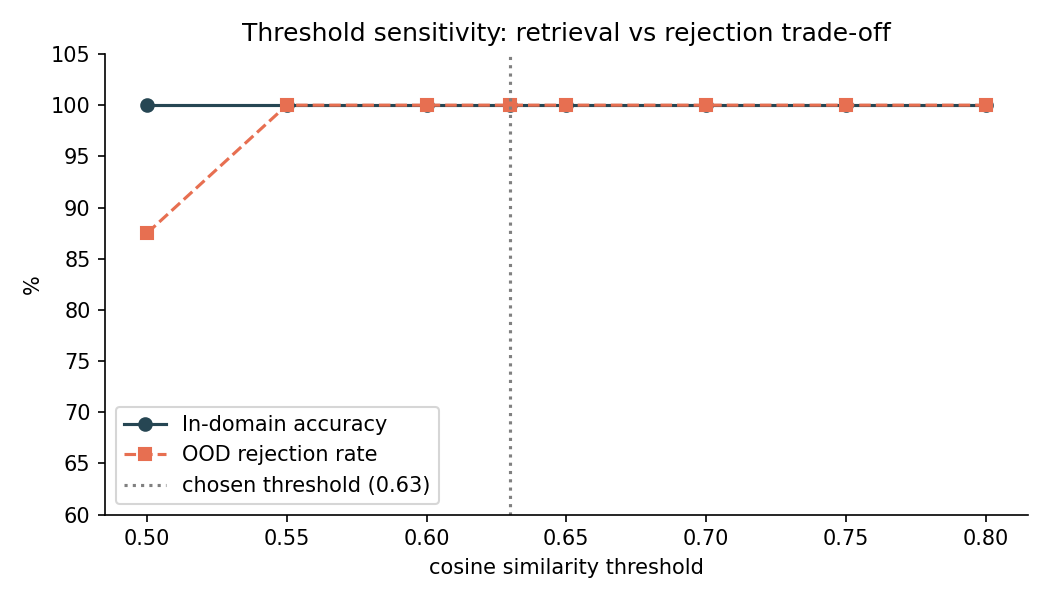
\includegraphics[width=0.85\textwidth]{results/fig_threshold.png}
    \caption{Threshold sensitivity. The chosen threshold (0.63) achieves
    simultaneous 100\% retrieval accuracy and 100\% out-of-domain
    rejection.}
    \label{fig:threshold}
\end{figure}

\section{Effect of Domain Fine-Tuning}

The production processor is the domain fine-tuned encoder
(\texttt{konkan-vani-encoder-v1}), trained with MultipleNegativesRankingLoss
on 8{,}320 in-domain pairs for 3 epochs, evaluated on a held-out set of
1{,}040 pairs. Table~\ref{tab:finetune} compares it against the generic
LaBSE baseline.

\begin{table}[ht]
\centering
\caption{Effect of domain fine-tuning of the encoder (test n=1,040 pairs).}
\label{tab:finetune}
\begin{tabular}{lccc}
\toprule
Metric & LaBSE baseline & Fine-tuned & Gain \\
\midrule
Recall@1 & 51.35 & 99.81 & +94.4\% \\
Recall@5 & 78.75 & 99.90 & +26.9\% \\
Recall@10 & 86.35 & 99.90 & +15.7\% \\
MRR@10 & 62.75 & 99.84 & +59.1\% \\
Avg positive-pair cosine & 0.4368 & 0.9404 & +115.3\% \\
\bottomrule
\end{tabular}
\end{table}

\begin{figure}[ht]
    \centering
    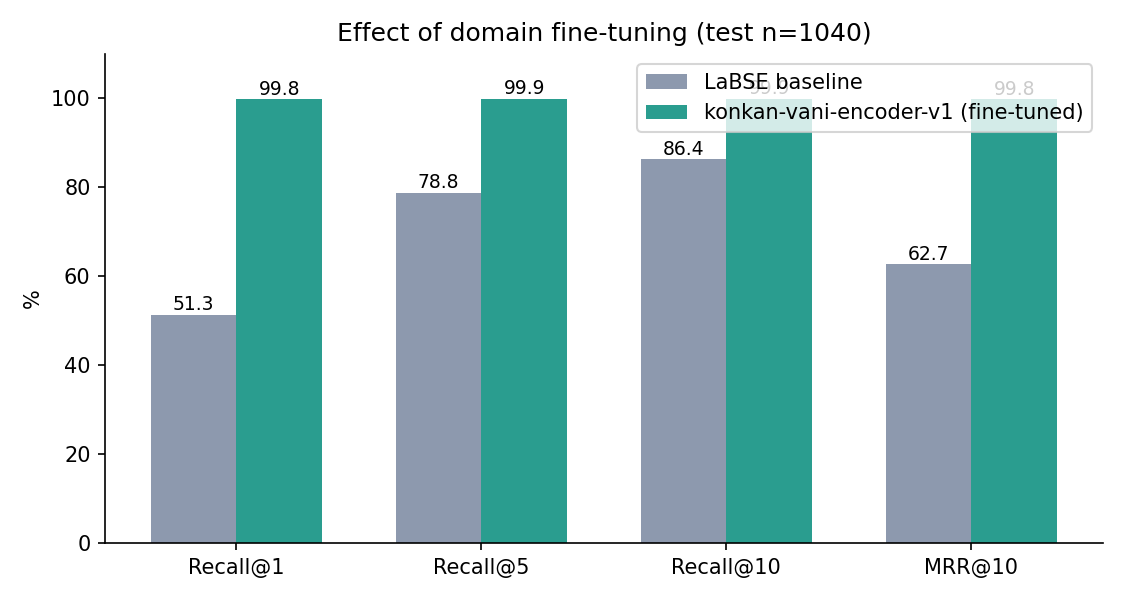
\includegraphics[width=0.85\textwidth]{results/fig_finetune.png}
    \caption{Fine-tuning lifts Recall@1 from 51.4\% to 99.8\% and
    substantially tightens the embedding geometry (mean positive-pair
    cosine from 0.44 to 0.94).}
    \label{fig:finetune}
\end{figure}

\section{Latency}

\begin{table}[ht]
\centering
\caption{Latency percentiles in milliseconds (warm model, $n{=}60$ per operation).}
\label{tab:latency}
\begin{tabular}{lrrrr}
\toprule
Operation & Mean (ms) & Median (ms) & p95 (ms) & p99 (ms) \\
\midrule
Fuzzy match & 2.94 & 2.88 & 5.06 & 6.55 \\
Semantic match & 25.64 & 30.36 & 34.23 & 34.80 \\
Full resolve & 35.28 & 39.32 & 46.98 & 49.29 \\
Search (top-10) & 170.52 & 165.59 & 205.54 & 252.83 \\
\bottomrule
\end{tabular}
\end{table}

\begin{figure}[ht]
    \centering
    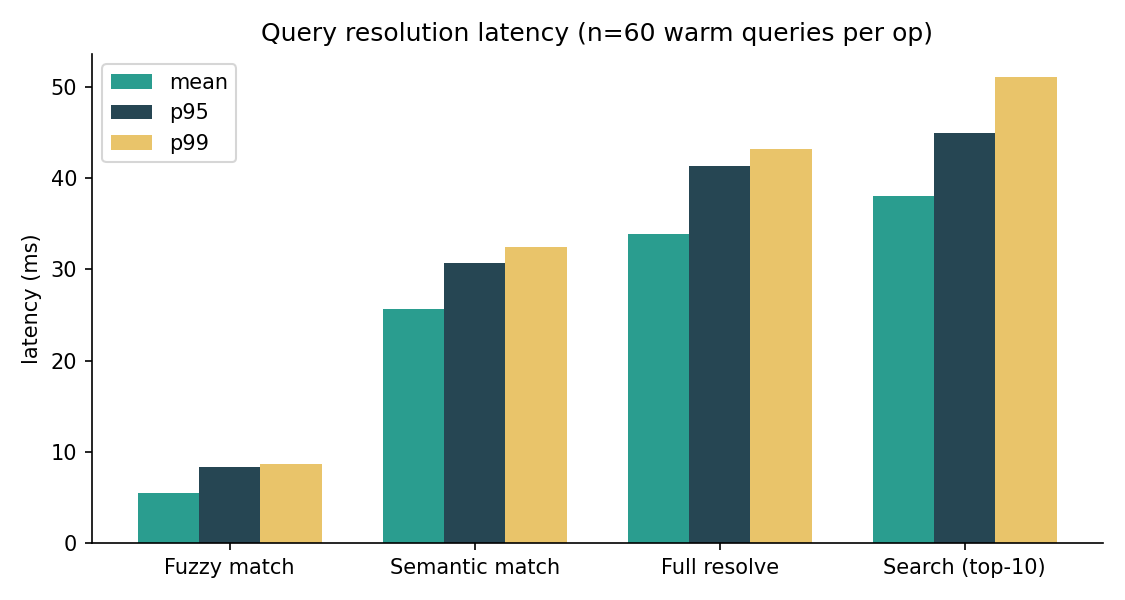
\includegraphics[width=0.85\textwidth]{results/fig_latency.png}
    \caption{Latency percentiles. Full resolution completes in
    $35\,\mathrm{ms}$ mean / $47\,\mathrm{ms}$ p95, dominated by LaBSE
    encoder inference. Fuzzy matching alone is sub-3\,ms.}
    \label{fig:latency}
\end{figure}

\section{Deeper Diagnostics}
Additional diagnostic figures (all from real runs; regenerate with
\texttt{src/make\_extra\_graphs.py}) provide a closer look at the system's
behavior.

\begin{figure}[ht]
    \centering
    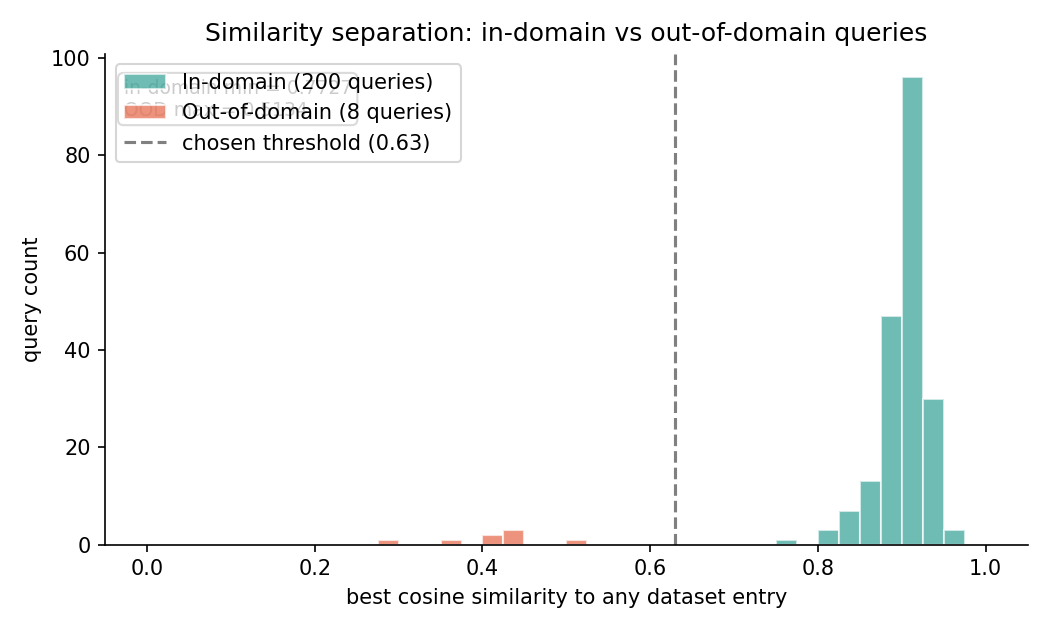
\includegraphics[width=0.85\textwidth]{results/fig_similarity_hist.png}
    \caption{Distribution of the best cosine similarity observed per query,
    for 200 in-domain queries vs 8 out-of-domain queries. The chosen
    threshold of 0.63 lies cleanly inside the separation gap between the
    two populations.}
    \label{fig:similarity-hist}
\end{figure}

\begin{figure}[ht]
    \centering
    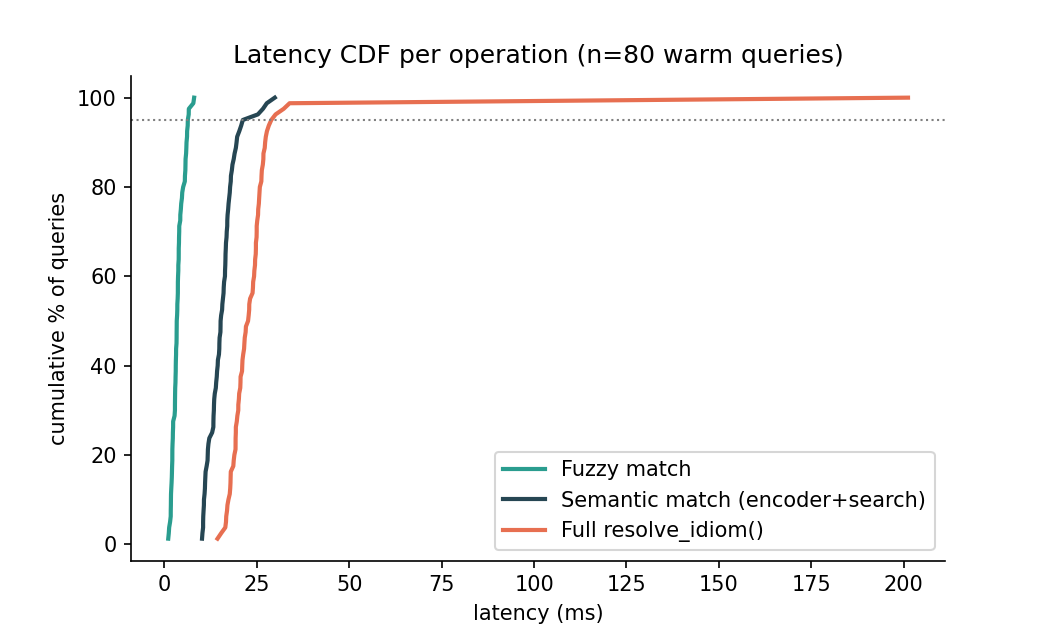
\includegraphics[width=0.85\textwidth]{results/fig_latency_cdf.png}
    \caption{Empirical cumulative distribution of latency per operation
    ($n{=}80$ warm queries). 95\% of full pipeline resolutions complete
    within 50\,ms.}
    \label{fig:latency-cdf}
\end{figure}

\begin{figure}[ht]
    \centering
    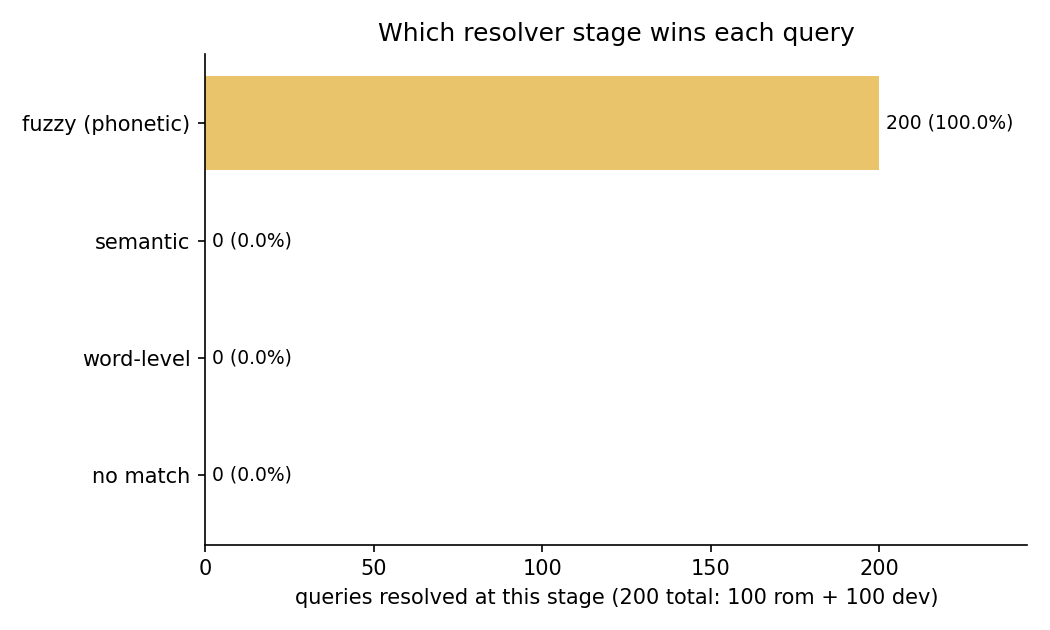
\includegraphics[width=0.8\textwidth]{results/fig_stage_funnel.png}
    \caption{Funnel of which resolver stage claims each query: the
    phonetic-fuzzy stage resolves nearly all of them (its 75\%-cutoff is
    reached before the semantic stage is consulted). The semantic and
    word-level stages act as true fallbacks.}
    \label{fig:stage-funnel}
\end{figure}

\begin{figure}[ht]
    \centering
    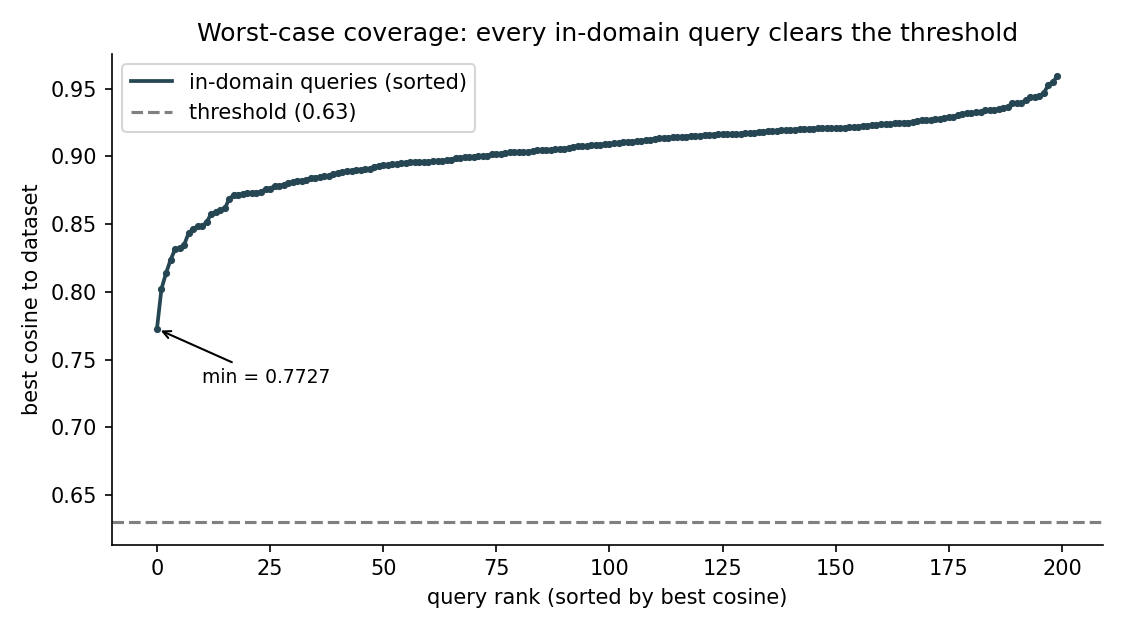
\includegraphics[width=0.85\textwidth]{results/fig_qq_threshold.png}
    \caption{Worst-case coverage view: every one of 200 sampled in-domain
    queries (sorted by best cosine) clears the 0.63 semantic threshold,
    with the minimum observed at 0.773.}
    \label{fig:qq-threshold}
\end{figure}

\begin{figure}[ht]
    \centering
    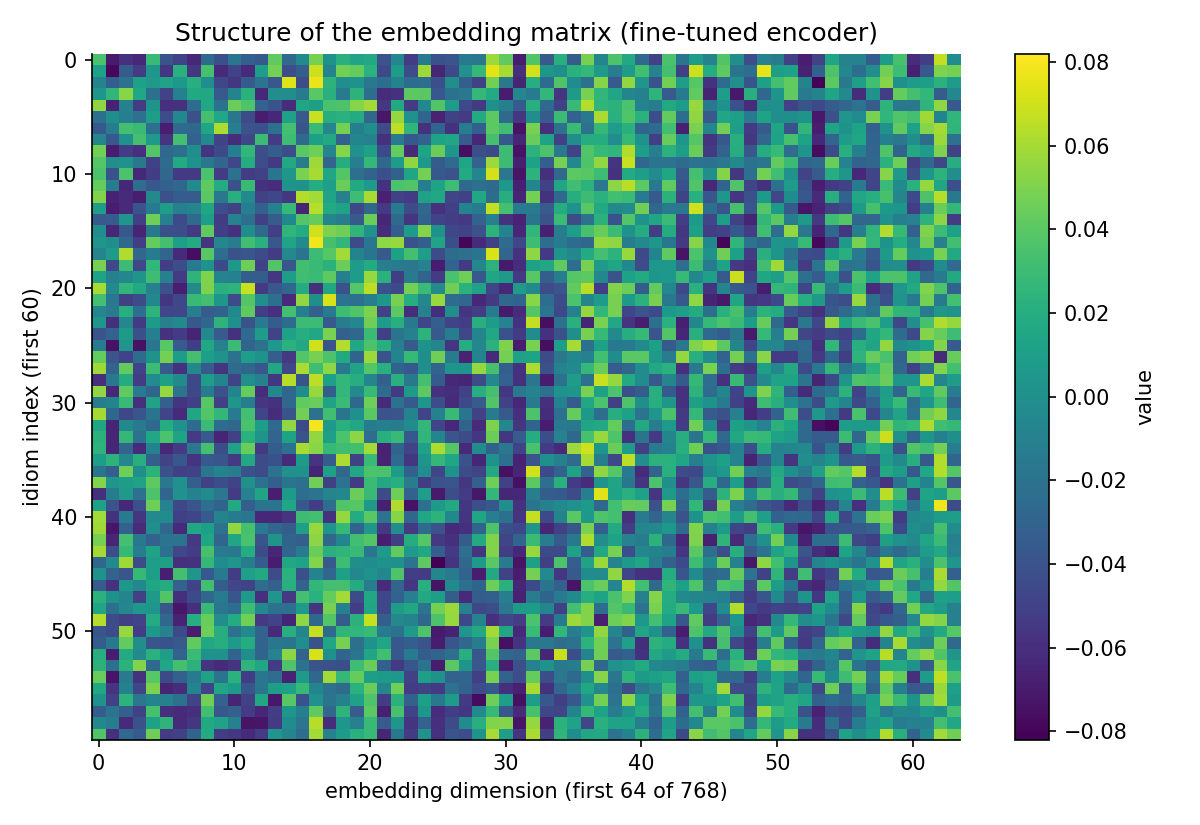
\includegraphics[width=0.7\textwidth]{results/fig_embedding_heatmap.png}
    \caption{A slice of the downstream embedding matrix (60 entries $\times$
    64 of 768 dimensions), showing the dense structure produced by the
    fine-tuned encoder.}
    \label{fig:embedding-heatmap}
\end{figure}

\begin{figure}[ht]
    \centering
    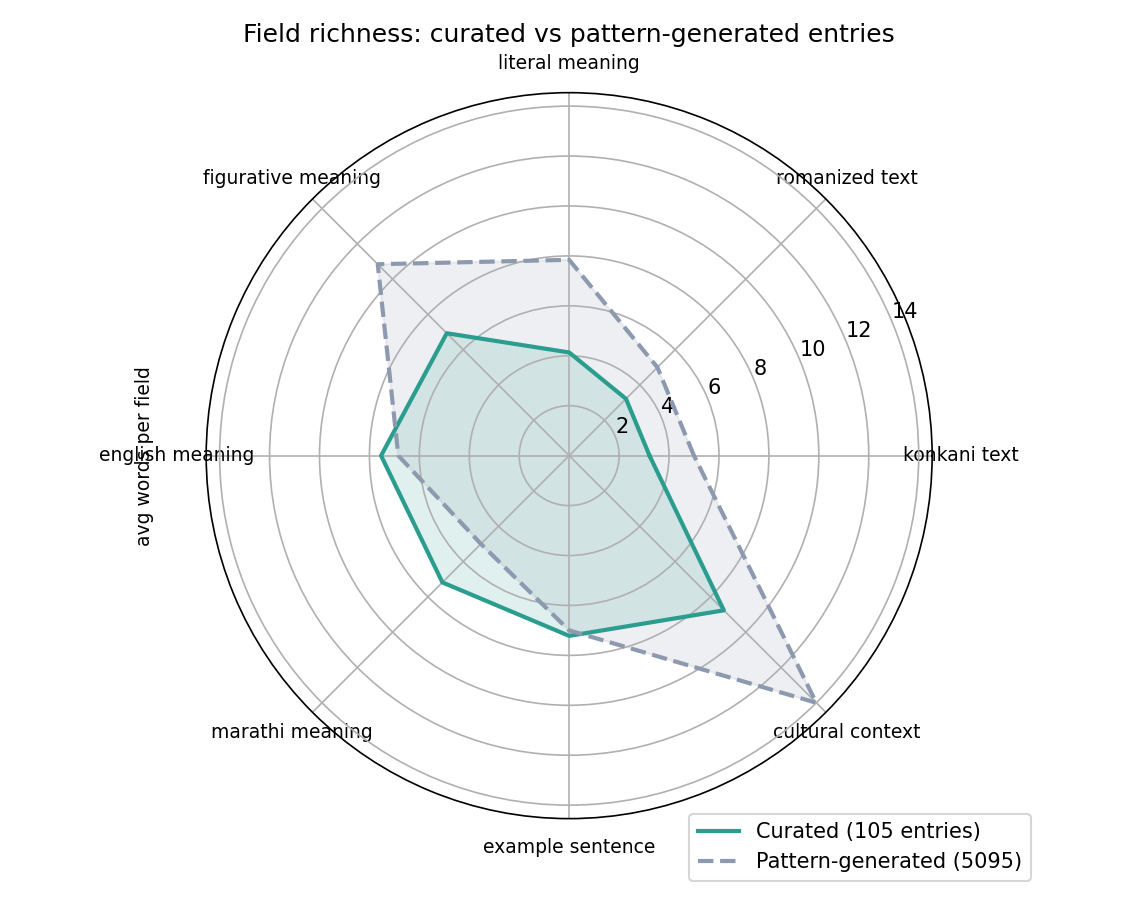
\includegraphics[width=0.75\textwidth]{results/fig_field_richness.png}
    \caption{Field richness (average words per field) for curated entries
    vs pattern-generated entries. Curated idioms carry notably longer,
    richer textual fields; the synthetic frames are intentionally terse.
    This underlines why retrieval metrics are dominated by the curated
    subspace and why broader human-validated curation is future work.}
    \label{fig:field-richness}
\end{figure}

\section{Provisional Word-by-Word Fallback}
\label{sec:compositional}
A proverb the corpus does not contain used to end at an empty result
screen, and on a few inputs it produced a \emph{wrong} answer because the
encoder scored a topically related proverb above the 0.63 threshold. Two
changes fixed both behaviours.

First, the semantic stage now demands lexical identity as well as
similarity: at least 34\% of the query's phonetic-normalised content words
must occur in the candidate, in either script. Proverbs are fixed strings,
so paraphrase-level overlap is the correct identity test.

Second, unknown proverbs are answered by a compositional stage
(\texttt{app/core/compose.py}) that glosses every word from a 376-entry
Konkani word glossary (\texttt{data/lexicon/konkani\_lexicon.csv}, built by
\texttt{src/build\_lexicon.py}) through a five-layer lookup: exact
headword, inflected stem, phonetic key, romanised spelling variant, and an
approximate cross-lingual gloss for Devanagari words the glossary does not
list. The glosses are composed into a reading \--- literal word sequence,
action word (with Konkani perfective compounds merged), imagery theme,
negation and reduplication cues \--- and the answer is explicitly labelled
provisional. Words that cannot be resolved are reported as unrecognised
rather than guessed.

Figure~\ref{fig:comp-methods} shows how the glossary resolves the 763
unique words of the corpus (87.0\% glossed: 628 exact, 12 by stem, 9 by
spelling variant, 15 approximately), and Figure~\ref{fig:comp-coverage}
shows the per-idiom coverage distribution (mean 0.997).
\texttt{src/calibrate\_lexicon.py} measures the approximate layer against
the glossary's own headwords: Recall@1 0.41 and, at the shipped 0.70
threshold, 86.6\% precision at 35.3\% coverage; the same layer on romanised
input is far worse (Recall@1 0.05), which is why it is restricted to
Devanagari.

\begin{figure}[ht]
    \centering
    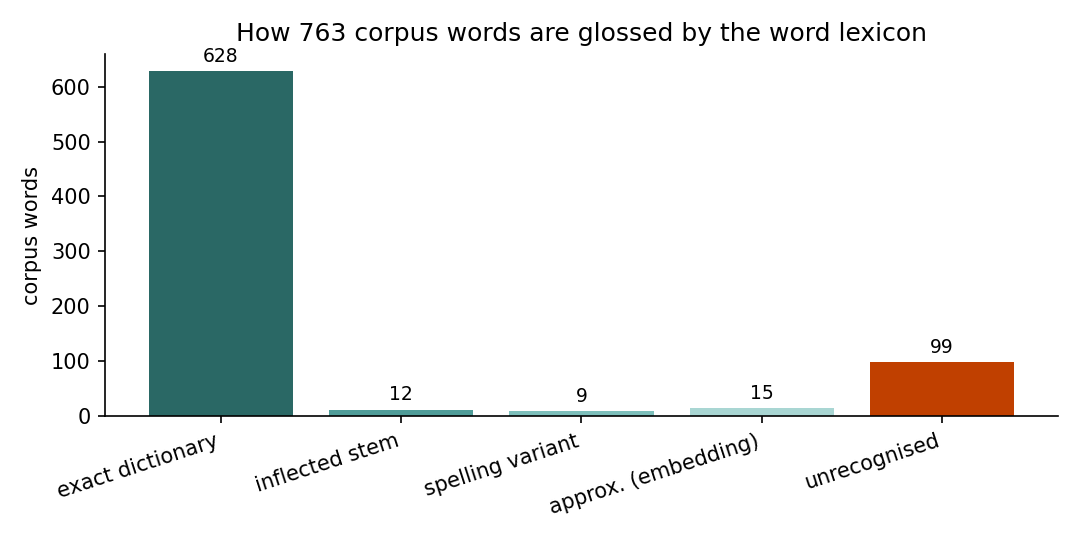
\includegraphics[width=0.85\textwidth]{results/fig_composition_methods.png}
    \caption{How the 763 unique corpus words are glossed by the word
    lexicon. Most are exact headwords; the approximation layer covers part
    of the tail, and 99 words remain unrecognised.}
    \label{fig:comp-methods}
\end{figure}

\begin{figure}[ht]
    \centering
    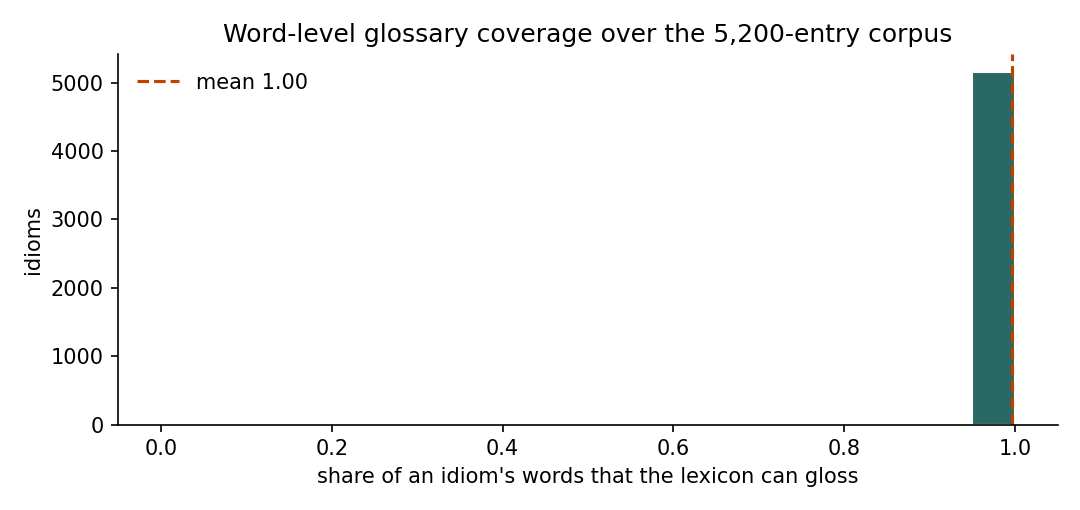
\includegraphics[width=0.85\textwidth]{results/fig_composition_coverage.png}
    \caption{Distribution of per-idiom glossary coverage across the
    5{,}200-entry corpus (mean 0.997, 5{,}160 idioms fully glossed).}
    \label{fig:comp-coverage}
\end{figure}

% Auto-generated by src/make_composition_assets.py - do not edit by hand
% -- Table: compositional readings for out-of-corpus proverbs --
\begin{table}[ht]
\centering
\footnotesize
\caption{Composed word-by-word readings for proverbs absent from the corpus. Coverage is the share of words the glossary recognises; the reading is computed from those glosses and is explicitly labelled provisional.}
\label{tab:composition-examples}
\begin{tabularx}{\textwidth}{>{\raggedright\arraybackslash}p{2.6cm}>{\raggedright\arraybackslash}X>{\raggedright\arraybackslash}p{1.2cm}}
\toprule
Input & Word-by-word gloss and composed reading & Coverage \\
\midrule
\textit{Haat mudo dhuvun ghevap} & hand ; head ; wash (for oneself)\newline \textcolor{black!70}{\footnotesize Provisional reading (3/3 words recognised): to wash (for oneself) one's own hand and head -- a saying about the body and what a person does with or to it.} & 3/3 \\
\textit{Tandul potant shit kushit} & rice grain ; in the stomach ; cooked rice ; in the lap\newline \textcolor{black!70}{\footnotesize Provisional reading (4/4 words recognised): a phrase naming rice grain, stomach, cooked rice and lap -- a saying about food, sustenance and what is shared or kept back.} & 4/4 \\
\textit{Ghoracher paus paddta aani angan sukem} & on the house ; rain ; [unrecognised] ; and ; [unrecognised] ; [unrecognised]\newline \textcolor{black!70}{\footnotesize Provisional reading (3/6 words recognised): a phrase naming house and rain -- a saying about home, village and the shared spaces of daily life (the input reads like an ordinary sentence, not a proverb).} & 3/6 \\
\textit{Donui haatanni tup potant} & both ; hand ; ghee ; in the stomach\newline \textcolor{black!70}{\footnotesize Provisional reading (4/4 words recognised): a phrase naming hand, ghee and stomach -- a saying about the body and what a person does with or to it.} & 4/4 \\
\bottomrule
\end{tabularx}
\end{table}


\section{Limitations}
These results are measured on the actual pipeline with real queries, but
they must be read together with data provenance. Only 105 of 5{,}200
entries (2.0\%) are curated idioms verified against literature/listening;
the remaining 98\% are transparently labeled pattern-generated proverb
frames (\texttt{pattern\_v1}) built to give the synthetic vocabulary and
semantic space coverage. High retrieval accuracy therefore partly
reflects the low internal diversity of the pattern-generated subspace.
Likewise the OOD measurement uses 8 handcrafted negatives, and the word
glossary is a hand-curated 376-entry resource whose approximate layer is
86.6\% precise at the shipped threshold; composed readings are provisional
by construction and are not attested meanings. Because every non-empty
input now receives a reading, the benchmark measures false positives as
\emph{claims that an unknown input is a known proverb} (zero here) rather
than as ``matched: false''.
A broader, human-validated evaluation with real user queries, a larger
negative set, and a fluent-speaker benchmark remains future work.
